\documentclass[11pt,a4paper]{article}

% Pacotes essenciais
\usepackage[utf8]{inputenc}
\usepackage[T1]{fontenc}
\usepackage{lmodern}
\usepackage[portuguese]{babel}
\usepackage{graphicx}
\usepackage{amsmath}
\usepackage{amsfonts}
\usepackage{amssymb}
\usepackage{float}
\usepackage{caption}
\usepackage{subcaption}
\usepackage{xcolor}
\usepackage{fancyhdr}
\usepackage{geometry}
\usepackage{titlesec}
\usepackage{lipsum}
\usepackage{cite}
\usepackage{booktabs}
\usepackage{array}
\usepackage{tikz}
\usepackage[hidelinks]{hyperref}

% Definição das cores
\definecolor{headercolor}{HTML}{b11116}
\definecolor{secondarycolor}{HTML}{3a5461}

% Configuração da página
\geometry{
    a4paper,
    top=2.8cm,
    bottom=2.5cm,
    left=2.5cm,
    right=2.5cm,
    headheight=1.2cm,
    headsep=0.5cm
}

% Configuração do cabeçalho
\pagestyle{fancy}
\fancyhf{}
\renewcommand{\headrulewidth}{0pt}
\renewcommand{\footrulewidth}{0.5pt}

\fancyhead[L]{%
    \begin{tikzpicture}[remember picture, overlay]
        \fill[headercolor] (current page.north west) rectangle ([yshift=-1.2cm]current page.north east);
        \node[anchor=west, inner sep=0pt] at ([xshift=1cm, yshift=-0.6cm]current page.north west) 
            {
\includegraphics[height=0.8cm]{imgs/base/fatec-rgt.png}};
        \node[anchor=east, inner sep=0pt] at ([xshift=-1cm, yshift=-0.6cm]current page.north east) 
            {
\includegraphics[height=0.9cm]{imgs/base/cps-logo.png}};
        \node[anchor=east, inner sep=0pt] at ([xshift=-2.8cm, yshift=-0.6cm]current page.north east) 
            {
\includegraphics[height=1.05cm]{imgs/base/governo-sp-secretaria-logo.png}};
    \end{tikzpicture}
}

\fancyfoot[L]{\footnotesize\textcolor{secondarycolor}{Faculdade de Tecnologia do Estado de São Paulo\\ fatecregistro.cps.sp.gov.br}}
\fancyfoot[R]{\thepage}

% Configuração dos títulos das seções
\titleformat{\section}
    {\normalfont\large\bfseries\color{secondarycolor}}
    {\thesection}{1em}{}

\titleformat{\subsection}
    {\normalfont\normalsize\bfseries\color{secondarycolor}}
    {\thesubsection}{1em}{}

% Informações do artigo
\title{\vspace{0.6cm}\textbf{\Large Plataforma IoT de monitoramento para criação de bubalinos}}
\author{
    Arthur Fukunaga Fagundes Nepomuceno$^{1}$,Matheus Ferrari Abrahão$^{2}$,\\Leonardo de Lima$^{3}$, Vinícius de Souza Camargo Costa $^{4}$ \\[0.3cm]
    \small
    $^{1}$Faculdade de Tecnologia do Estado de São Paulo \\
    $^{2}$Universidade de São Paulo \\
    $^{3}$Instituto de Pesquisas Tecnológicas \\[0.2cm]
    {\itshape arthur.nepomuceno@aluno.cps.sp.gov.br, matheus.abrahao@aluno.cps.sp.gov.br,}\\ {\itshape leonardo.lima3@aluno.cps.sp.gov.br, vinicius.costa16@aluno.cps.sp.gov.br}
}
\date{}

\begin{document}

% Força o cabeçalho em todas as páginas
\pagestyle{fancy}

\maketitle
\thispagestyle{fancy}

% Abstract
\section*{Abstract}

 Buffalo farming has become an important livestock activity in Brazil, particularly in the Vale do Ribeira region, which accounts for approximately 42\% of São Paulo State's production. The adoption of this practice serves as an economic and social driver, generating income, employ- ment, and diversifying local production. With the advancement of digital technologies, new opportunities arise to integrate innovative solutions into agricultural management, contributing to production efficiency and animal welfare. This project proposes the development of an in- telligent monitoring system designed to track the stress levels and location of buffaloes in open pastures. The system consists of electronic collars equipped with physiological sensors and GPS modules, connected to an Internet of Things (IoT) infrastructure responsible for collecting and transmitting data to a cloud-based platform. This structure is supported by communication towers that create a "virtual fence," enabling continuous tracking of the animals and the auto- matic generation of alerts in cases of behavioral or physiological anomalies. A web and mobile interface will allow farmers to visualize the collected data in real time, optimizing herd manage- ment and promoting a more technological, sustainable production aligned with the Sustainable Development Goals (SDGs), particularly SDG 2 (Zero Hunger and Sustainable Agriculture) and SDG 12 (Responsible Consumption and Production).

\vspace{0.3cm}
\noindent\textit{\textbf{Palavras-chave:}} Buffalo farming, Animal welfare, Smart tracking, Internet of Things, Realtime Monitoring.

\vspace{0.5cm}
\noindent\rule{\textwidth}{0.5pt}
\vspace{0.5cm}

% Resumo
\section*{Resumo}

A bubalinocultura tornou-se uma importante atividade pecuária no Brasil, com destaque para o Vale do Ribeira, que apresenta cerca de 42\% da produção do estado de São Paulo. A adoção dessa prática representa um motor econômico e social, gerando renda, empregos e diversificando a produção local. Com o avanço das tecnologias digitais, surge a oportunidade de integrar soluções inovadoras à gestão agropecuária, contribuindo para a eficiência produtiva e o bem estar animal. O presente projeto propõe o desenvolvimento de um sistema de monitoramento inteligente destinado ao acompanhamento do estresse e da localização de bubalinos em pasto aberto. O sistema é composto por coleiras eletrônicas equipadas com sensores fisiológicos e módulos GPS, conectadas a uma infraestrutura loT (Internet das Coisas) que realiza a coleta e o envio de dados a uma plataforma em nuvem. Essa estrutura é apoiada por torres de comunicação que formam uma "cerca virtual", permitindo o rastreamento contínuo dos animais e a geração de alertas automáticos em casos de anomalias comportamentais ou fisiológicas. A interface web e mobile permitirá ao pecuarista visualizar, em tempo real, as informações coletadas, otimizando o manejo do rebanho e promovendo uma produção mais tecnológica, sustentável e alinhada aos Objetivos de Desenvolvimento Sustentável, especialmente o ODS 2 (Fome Zero e Agricultu a Sustentável) e o ODS 12 (Consumo e Produção responsáveis).

\vspace{0.3cm}
\noindent\textit{\textbf{Palavras-chave:}} Bubalinocultura, Bem-estar, Rastreamento inteligente, Internet das Coisas, Monitoramento em tempo real.

\vspace{0.5cm}
\noindent\rule{\textwidth}{0.5pt}
\vspace{0.5cm}

% Introdução
\section{Introdução}

A bubalinocultura tem se destacado no agronegócio mundial devido à sua relevância econômica e nutricional e produtiva. Em 2023, a produção global de leite de búfala atingiu aproximadamente 147 milhões de toneladas, demonstrando a crescente importância da atividade no cenário inter nacional [1]. No Brasil, o rebanho bubalino também apresenta expansão significativa, alcançando cerca de 1,8 milhão de cabeças em 2024, distribuídas em diferentes estados do país [2].

A criação de búfalos possui grande importância para o atendimento da demanda alimentar, especialmente na produção de leite e carne, além de contribuir para o desenvolvimento econômico regional [3]. Apesar do potencial produtivo da bubalinocultura, o setor ainda enfrenta desafios importantes para garantir eficiência, produtividade e qualidade na produção leiteira. Entre esses desafios, o estresse térmico destaca-se como um dos principais fatores limitantes da atividade.

Pesquisas indicam que o estresse térmico pode reduzir os teores de gordura e proteína do leite, diminuir a taxa de prenhez e ocasionar perdas produtivas significativas [4]. Estudos apontam reduções de produtividade entre 15\% e 20\%, além de prejuízos econômicos superiores a R\$ 700,00 por animal ao ano no Brasil [5]. Nesse contexto, torna-se essencial o desenvolvimento de estratégias capazes de minimizar os impactos do calor sobre os animais, promovendo maior bem-estar, sustentabilidade e rentabilidade ao setor.

Além das questões relacionadas ao ambiente e ao manejo, observa-se também uma limitação
tecnológica significativa na bubalinocultura. Diferentemente da bovinocultura leiteira, que pos
sui ampla oferta de ferramentas digitais de monitoramento e gestão, a produção bubalina ainda
carece de soluções específicas para suas características fisiológicas e produtivas. Essa ausência
de ferramentas específicas compromete o monitoramento zootécnico e dificulta a implementação
de práticas de Pecuária de Precisão voltadas à bubalinocultura.   

Com o objetivo de compreender as práticas de manejo adotadas na produção leiteira bu
balina, foi realizada uma pesquisa qualitativa em uma propriedade localizada na cidade de
Registro, no Vale do Ribeira. A coleta de dados ocorreu por meio da aplicação de um ques
tionário composto por 20 questões discursivas, permitindo compreender as particularidades da
rotina produtiva e os desafios enfrentados pelos produtores.

A pesquisa de campo realizada em uma propriedade bubalina localizada em Registro-SP
evidenciou que o monitoramento do estresse animal ocorre predominantemente por observação
comportamental, sendo identificado apenas em situações de agressividade ou resistência durante
a ordenha. Além disso, observou-se ausência de ferramentas tecnológicas específicas para acom-
panhamento fisiológico dos animais, bem como elevada dependência de estratégias naturais de
termorregulação, como acesso à água e áreas sombreadas. Esses fatores reforçam a necessidade
do desenvolvimento de soluções tecnológicas adaptadas às particularidades da bubalinocultura
regional. O fazendeiro entrevistado, além disso, demonstrou interesse na utilização de sistemas
digitais capazes de auxiliar no monitoramento produtivo, sanitário e reprodutivo dos animais. A
pesquisa também evidenciou a necessidade de adaptação das funcionalidades tecnológicas às de
mandas reais do manejo bubalino, especialmente em relação ao monitoramento comportamental
e ambiental dos animais.

Além dos desafios produtivos e tecnológicos identificados na pesquisa de campo, a necessidade
de modernização da bubalinocultura também está alinhada aos Objetivos de Desenvolvimento
Sustentável (ODS), especialmente ao ODS 2 (Fome Zero e Agricultura Sustentável) e ao ODS
12 (Consumo e Produção Responsáveis). Nesse cenário, torna-se necessário reduzir desperdícios,
otimizar recursos produtivos, melhorar o bem-estar animal e ampliar a oferta de proteínas de
alta qualidade.

O uso de sensores, geolocalização, computação em nuvem e Internet das Coisas (IoT) pode
contribuir significativamente para o monitoramento fisiológico e comportamental dos animais,
permitindo identificar situações de estresse térmico, padrões de deslocamento e necessidades
relacionadas à disponibilidade de água e sombra.

Diante desse contexto, este estudo propõe o desenvolvimento e a validação de uma plataforma
de baixo custo baseada em Internet das Coisas (IoT) para aplicação na bubalinocultura de
precisão. A plataforma tem como objetivo coletar, processar e analisar dados fisiológicos e
comportamentais dos animais de forma automatizada, utilizando sensores para monitoramento
de temperatura, frequência cardíaca e geolocalização. Os dados obtidos serão armazenados e
processados em nuvem, permitindo análises em tempo real e oferecendo suporte à tomada de
decisão.

A principal contribuição deste estudo consiste no desenvolvimento de uma ferramenta aces
sível, específica e adaptada à realidade da bubalinocultura, especialmente para auxiliar no mo
nitoramento do estresse térmico. Espera-se que a adoção dessa tecnologia contribua para o
aumento da produtividade, melhoria do bem-estar animal e fortalecimento da sustentabilidade
e competitividade do setor bubalino.

% Objetivo
\section{Objetivo}

Desenvolver e validar uma Arquitetura de Internet das Coisas (IoT) e Computação em Nuvem
para a Bubalinocultura de Precisão, visando o monitoramento contínuo do bem-estar animal
em fazendas de pequeno e médio porte do Vale do Ribeira. Especificamente, o estudo busca
correlacionar indicadores fisiológicos (frequência cardíaca e temperatura corporal) com o nível de
estresse bubalino para a otimização do manejo e a preservação da qualidade dos produtos.Para
atingir o objetivo geral, foram definidos os seguintes objetivos específicos:

\begin{itemize}
    \item  Propor e implementar um protocolo de aquisição de dados de geolocalização com latência
máxima de 5 minutos, garantindo a rastreabilidade individual dos animais em ambiente
de fazenda;
    \item  Projetar e construir um protótipo de coleira inteligente baseado em ESP32 que integre
sensores de frequência cardíaca e temperatura corporal para coleta de dados fisiológicos
em campo;
    \item  Validar a acurácia da medição da frequência cardíaca do bubalino com erro máximo de 5
batimentos por minuto;
    \item  Determinar a temperatura corporal com margem de erro máxima de 2 graus e correlaci
onar a temperatura superficial medida pela coleira com a temperatura de referência para
monitoramento do estresse térmico;
    \item Adaptar o software PRTG (Paessler Router Traffic Grapher) para o monitoramento dos
dados obtidos pelas coleiras;
    \item Estabelecer uma infraestrutura de comunicação de Longa Distância e Baixo Consumo de
Energia no ambiente rural para garantir a conectividade contínua e a transmissão dos
dados das coleiras para a nuvem.
\end{itemize}

% Estado da Arte
\section{Estado da Arte}

O avanço da Pecuária de Precisão tem impulsionado o desenvolvimento de sistemas inteligentes
voltados ao monitoramento animal, especialmente por meio de tecnologias baseadas em Internet
das Coisas (IoT), dispositivos inteligentes acoplados aos animais e comunicação sem fio. Essas
soluções buscam ampliar a capacidade de acompanhamento do comportamento, da saúde e do
bem-estar dos animais em tempo real, permitindo intervenções mais rápidas e maior eficiência
produtiva. Entretanto, grande parte das pesquisas concentra-se na bovinocultura, havendo ainda
uma escassez significativa de estudos direcionados especificamente à bubalinocultura, apesar das
particularidades fisiológicas e comportamentais dessa espécie. Com o objetivo de contextuali
zar esta proposta e identificar lacunas científicas relevantes, foram selecionados três trabalhos
representativos do estado da arte em monitoramento inteligente aplicado à pecuária.

O estudo de [6] apresenta uma revisão sistemática sobre tecnologias vestíveis aplicadas à Pe
cuária de Precisão. Os autores analisam diferentes sensores empregados em colares inteligentes,
incluindo acelerômetros, GPS e microfones, utilizados para monitoramento de atividade, rumi
nação e detecção de cio em bovinos leiteiros. O trabalho evidencia o avanço das tecnologias de
monitoramento animal e demonstra a consolidação dos sistemas IoT no contexto da produção
leiteira. Contudo, os próprios autores destacam como limitação a forte concentração das vali
dações experimentais em bovinos, indicando a ausência de estudos robustos voltados a outras
espécies ruminantes, como os bubalinos. Além disso, a revisão aponta que o monitoramento
fisiológico contínuo, especialmente de parâmetros relacionados ao estresse térmico e frequência
cardíaca, ainda representa um desafio tecnológico relevante.

Em uma abordagem mais aplicada, [7] desenvolveram um sistema IoT de baixo custo voltado
ao rastreamento animal em sistemas de pastoreio. A proposta baseia-se em dispositivos vestíveis
equipados com GPS e comunicação sem fio para implementação de cercas virtuais (geofencing).
Os resultados demonstraram a viabilidade técnica e econômica da solução para monitoramento
espacial do rebanho. Entretanto, embora eficiente para localização geográfica, o sistema não
contempla parâmetros fisiológicos ou indicadores de bem-estar animal, limitando sua aplicação
em cenários que demandam monitoramento integrado da saúde dos animais.

Entre os estudos mais próximos da presente proposta destaca-se o trabalho de [8], que desenvolveu um protótipo IoT especificamente direcionado ao monitoramento de búfalos. O sistema
integra sensores de temperatura corporal, frequência cardíaca e GPS, com transmissão de dados
via GSM/GPRS. A pesquisa demonstra a viabilidade da coleta remota de parâmetros fisiológicos
em bubalinos e representa um avanço importante para a aplicação da Pecuária de Precisão nessa
espécie. Contudo, o estudo apresenta limitações relacionadas à ausência de validação experimental rigorosa dos sensores utilizados, especialmente no que se refere à precisão da aferição da
frequência cardíaca em condições reais de campo. Além disso, aspectos como autonomia energética, robustez operacional e confiabilidade metrológica do dispositivo não foram explorados de
forma aprofundada.

A análise comparativa dos trabalhos correlatos evidencia que a literatura atual apresenta
três características principais: (i) predominância de pesquisas voltadas à bovinocultura; (ii) foco majoritário em monitoramento comportamental ou geoespacial; e (iii) carência de validações experimentais robustas envolvendo parâmetros fisiológicos em bubalinos. Embora existam
soluções capazes de integrar sensores fisiológicos e geolocalização, observa-se que muitas permanecem em nível de prototipagem inicial, sem avaliações metrológicas detalhadas da confiabilidade dos dados coletados.

Nesse contexto, o presente trabalho diferencia-se por propor um sistema de monitoramento
inteligente especificamente voltado à bubalinocultura, integrando sensores fisiológicos, térmicos
e de geolocalização em uma única arquitetura IoT. Além da prototipagem do dispositivo, a
proposta concentra-se na validação experimental da acurácia dos sensores empregados, estabelecendo critérios quantitativos de erro e confiabilidade. Dessa forma, o trabalho busca contribuir
não apenas com uma solução tecnológica funcional, mas também com evidências científicas sobre
a precisão e aplicabilidade do sistema em condições reais de uso, preenchendo uma lacuna ainda
pouco explorada na literatura da Pecuária de Precisão aplicada a bubalinos.

% Metodologia
\section{Metodologia}

Esta seção apresenta os procedimentos metodológicos adotados para o desenvolvimento e validação da plataforma IoT proposta para aplicação na bubalinocultura de precisão. Inicialmente,
é realizada a caracterização da pesquisa, definindo sua natureza, abordagem e objetivos experimentais. Em seguida, são descritos os componentes que compõem a arquitetura geral do sistema,
incluindo o desenvolvimento do protótipo da coleira inteligente, a infraestrutura de comunicação IoT e os módulos de software responsáveis pela aquisição, processamento, armazenamento
e visualização dos dados.

Por fim, são detalhadas as funcionalidades da API REST, do aplicativo mobile, da plataforma
web/desktop e dos dashboards utilizados para monitoramento em tempo real das informações
fisiológicas e geoespaciais dos animais. A metodologia adotada visa garantir a robustez técnica,
a aplicabilidade prática e a relevância científica da solução proposta, alinhando-se aos objetivos
de desenvolvimento tecnológico e à validação experimental dos sensores empregados.


\subsection{PESQUISA DE CAMPO}

Esta pesquisa caracteriza-se como aplicada, de abordagem quantitativa e caráter experimental,
tendo como objetivo o desenvolvimento e a validação de uma plataforma baseada em Internet
das Coisas (IoT) para monitoramento fisiológico e geoespacial de bubalinos. O estudo envolve
atividades de prototipagem eletrônica, implementação de infraestrutura de comunicação sem fio,
desenvolvimento de software e validação experimental dos sensores empregados em condições
reais de campo. A pesquisa de campo foi conduzida em uma propriedade bubalina localizada no
Vale do Ribeira, onde foram coletados dados sobre as práticas de manejo, condições ambientais
e desafios enfrentados pelos produtores.

O questionário aplicado durante a pesquisa de campo foi estruturado em 20 questões discursivas, abordando temas como monitoramento do estresse animal, monitoramento fisiológico
(temperatura corporal e frequência cardíaca), geolocalização, práticas de manejo e uso de tecnologias na fazenda. As respostas obtidas permitiram compreender as particularidades da rotina
produtiva, os desafios enfrentados pelos produtores e as lacunas tecnológicas existentes, especialmente no que se refere ao monitoramento fisiológico dos animais. Os dados coletados foram
analisados qualitativamente para identificar padrões e insights relevantes para o desenvolvimento
do protótipo da coleira inteligente e a definição dos requisitos técnicos do sistema IoT proposto,
sendo estes apresentados na Tabela 1.

Na categoria de monitoramento do estresse animal, a pesquisa evidenciou que a identificação
do estresse ocorre predominantemente por observação comportamental durante a ordenha, considerando sinais como agressividade, resistência ao manejo e agitação. 


\begin{table}[htbp]
\centering
\caption{Análise qualitativa da pesquisa de campo}
\label{tab:analise_qualitativa}
\begin{tabular}{|l|l|l|}
\hline
\textbf{Categoria} & \textbf{Evidência observada} & \textbf{Implicação no sistema} \\ \hline
Estresse & Identificação visual & Necessidade de monitoramento automático \\ \hline
Temperatura & Uso de água e lama & Impermeabilização da coleta \\ \hline
Monitoramento & Ausência de sensores & Lacuna tecnológica \\ \hline
Rotina & Ordenha diaria & Janela de coleta de dados \\ \hline
\end{tabular}
\end{table}

Não foram identificados mecanismos automatizados ou métricas fisiológicas objetivas para monitoramento contínuo do
bem-estar animal. Com relação a categoria Temperatura, os produtores relataram a utilização
de estratégias naturais de termorregulação, como acesso à água, lama e áreas sombreadas, para
mitigar os efeitos do calor sobre os animais. Esses fatores influenciaram diretamente os requisitos de engenharia do protótipo da coleira inteligente, especialmente em relação à necessidade de
impermeabilização e resistência ambiental dos dispositivos. Além disso, observou-se ausência de
sensores ou dispositivos eletrônicos aplicados ao monitoramento animal, indicando uma lacuna
tecnológica significativa e reforçando a necessidade de desenvolvimento de soluções específicas
para a bubalinocultura. Por fim, a rotina diária da fazenda, especialmente os procedimentos
relacionados à ordenha, foram identificados como momentos críticos para a coleta de dados, definindo uma janela temporal específica para o monitoramento e análise dos parâmetros fisiológicos
dos animais. É durante a ordenha que os procedimentos veterinários são realizados, o que torna
esse período ideal para a coleta de dados sem interferir no manejo e garantindo a segurança e o
conforto dos animais.

\subsection{ARQUITETURA GERAL DO SISTEMA}

O projeto visa construir um protótipo de coleira inteligente para o monitoramento do estresse
e geolocalização dos bubalinos pela captura de dados por meio de sensores, utilizando técnicas
de Internet das Coisas e Computação em Nuvem. O sistema é composto por três componentes
principais: um aplicativo mobile, uma aplicação web/desktop e uma API que conecta os dados
com a nuvem.

O funcionamento da solução proposta pode ser visualizado na Figura 1. A arquitetura
proposta é composta por quatro camadas principais: aquisição de dados, comunicação, processamento em nuvem e visualização. Na camada de aquisição, as coleiras inteligentes realizam
a coleta de parâmetros fisiológicos e geoespaciais dos animais. Os dados são transmitidos por
meio de comunicação LoRaWAN para um gateway central conectado à infraestrutura de nuvem. Na camada de processamento, a API REST realiza a integração entre o banco de dados,
o software PRTG e os módulos de Inteligência Artificial responsáveis pela análise dos indicadores de estresse animal. Por fim, os dados processados são disponibilizados em interfaces web e
mobile para acompanhamento em tempo real pelo produtor rural. A seguir, são detalhados os
componentes identificados de A a G e o fluxo de funcionamento do sistema, conforme ilustrado
na Figura 1.

\begin{figure}[H]
    \centering
    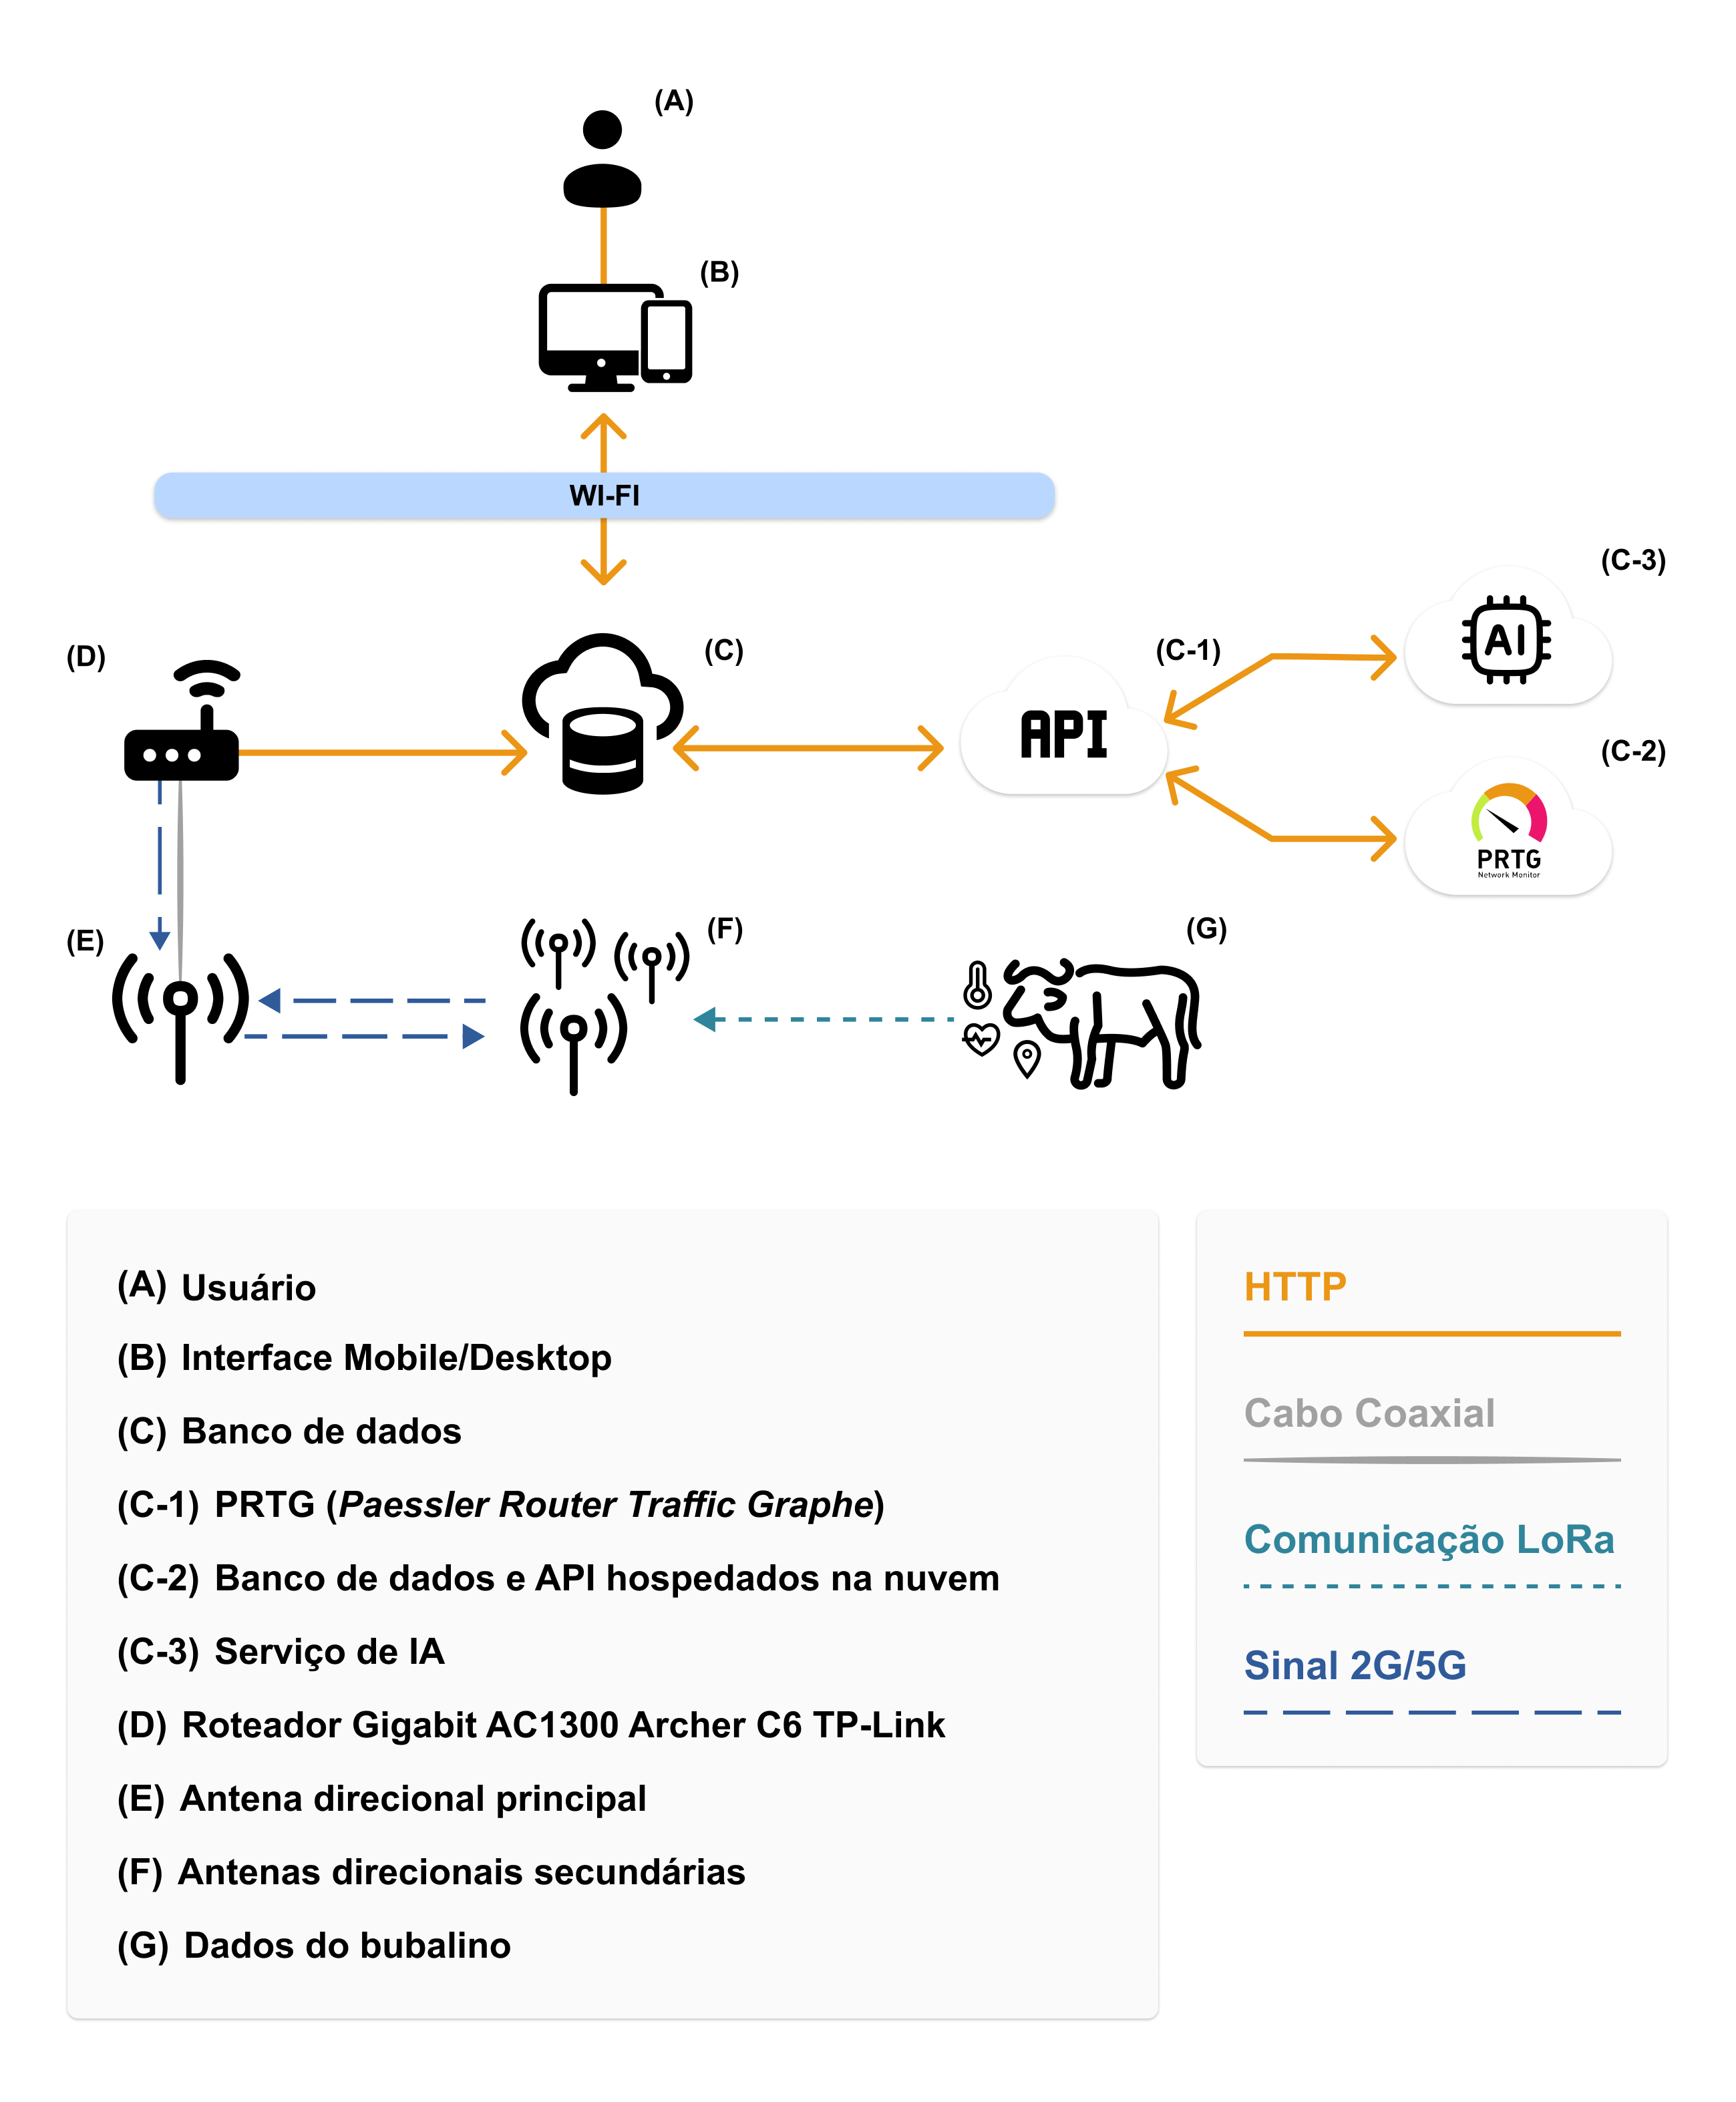
\includegraphics[width=0.9\textwidth]{imgs/bubatag/DIAGRAMA DE REDE - ARTIGO.png}
    \caption{Fluxograma de funcionamento da rede de informações do sistema de monitoramento inteligente para bubalinos.}
    \label{fig:fluxograma_bubalinos}
\end{figure}

O usuário (A) acessa as informações do sistema por meio das interfaces web e mobile (B),
desenvolvidas para permitir a visualização de relatórios, dashboards e alertas em tempo real,
facilitando a interpretação dos dados coletados no ambiente rural.

O armazenamento e processamento das informações são realizados em um banco de dados
hospedado em servidor na nuvem (C), responsável por centralizar, tratar e distribuir os dados
recebidos das coleiras inteligentes. A integração entre os diferentes módulos do sistema ocorre
por meio de uma API REST (C-1), encarregada de realizar o tráfego de informações entre
o banco de dados, o software PRTG (Paessler Router Traffic Grapher, C-2) e os serviços de
Inteligência Artificial (C-3).

O software PRTG é utilizado para monitorar a disponibilidade da infraestrutura de rede
e acompanhar o desempenho da comunicação entre os dispositivos distribuídos na fazenda.
Paralelamente, os módulos de Inteligência Artificial realizam o processamento dos parâmetros
fisiológicos coletados pelos sensores, permitindo identificar padrões de comportamento e possíveis
situações de estresse animal, além da geração automatizada de relatórios.

A infraestrutura de comunicação é composta por um roteador TP-Link CPE210 (D), responsável pelo envio dos dados captados pelas antenas para a nuvem por meio de diferentes
protocolos de transmissão. O sistema também utiliza uma antena direcional principal (E), encarregada da recepção e emissão dos sinais de comunicação, garantindo ampla cobertura da área
monitorada. Além disso, antenas direcionais secundárias (F) são empregadas para concentrar o
sinal em regiões específicas da propriedade, aumentando o alcance e a eficiência da transmissão
dos dados.

Por fim, os dados coletados pelas coleiras inteligentes (G) incluem informações relacionadas à
temperatura corporal, localização geográfica, nível de atividade e demais indicadores fisiológicos dos bubalinos, possibilitando o monitoramento contínuo do bem-estar animal e das condições
ambientais da fazenda.

\subsection{DESENVOLVIMENTO DO PROTÓTIPO DA COLEIRA INTELIGENTE E
COMUNICAÇÃO IoT}

Para a validação da construção do protótipo da coleira, foi realizada uma pesquisa para identificar quais periféricos seriam necessários, sendo estes: um microcontrolador ESP32, escolhido
pelo baixo custo em comparação a outros dispositivos disponíveis no mercado e pela disponibilidade das tecnologias Wi-Fi e Bluetooth; um sensor de batimentos cardíacos modelo XD-58C,
selecionado pelo seu bom custo-benefício; e um sensor de temperatura infravermelho modelo
MLX90614, adotado devido à precisão na medição sem contato direto com a pele do animal,
o que garante menor oscilação nos dados e maior precisão nas informações obtidas. Para captação de dados de monitoramento da coleira será utilizado o software comercial PRTG (C-2)
especializado em monitoramento de redes e infraestrutura de TI em conjunto com um roteador
Wireless Gigabit AC1300 Archer C6 TP-Link, 4 antenas direcionais distribuídas no pasto com
um repetidor em 3 delas, e uma delas será responsável pelo acoplamento do roteador. Para
manter o roteador e os repetidores ligados será utilizado um kit solar independente para cada
dispositivo em conjunto com uma bateria de 12V e um regulador de tensão Buck-Boost DC-DC.

A estrutura física da coleira inteligente será projetada visando minimizar impactos no comportamento e no bem-estar dos bubalinos durante o monitoramento contínuo. O dispositivo
será fixado ao animal por meio de uma coleira ajustável confeccionada em material resistente e
impermeável, permitindo adaptação a diferentes portes de animais e garantindo estabilidade durante a movimentação em campo. Considerando as características comportamentais da espécie
e os resultados obtidos na pesquisa de campo, o encapsulamento eletrônico da coleira será desenvolvido com proteção contra água, lama e umidade, possibilitando seu funcionamento mesmo
em situações de imersão parcial dos animais em tanques e áreas alagadas.

Além disso, o protótipo será projetado para possuir baixo peso, reduzindo desconfortos e
interferências na rotina dos animais durante atividades como pastejo, deslocamento e ordenha.
A autonomia energética do sistema será garantida por meio de baterias recarregáveis de baixo
consumo associadas à comunicação LoRaWAN, permitindo operação contínua por longos períodos sem necessidade de manutenção frequente. Dessa forma, busca-se garantir não apenas
a viabilidade técnica do sistema, mas também sua aplicabilidade prática em ambientes rurais
extensivos característicos da bubalinocultura.

O sistema será estruturado e funcionará da seguinte forma: inicialmente, será realizada uma
verificação das condições do pasto da fazenda, com o objetivo de identificar obstáculos como
árvores ou relevos que possam interferir na propagação do sinal entre as antenas, os repetidores
e o gateway central (D).

Para garantir comunicação de longa distância com baixo consumo de energia, será utilizado
uma comunicação LoraWAN entre as coleiras inteligentes e o gateway central (roteador, D).
A utilização do protocolo LoRaWAN foi definido devido à sua capacidade de comunicação de
longa distância com baixo consumo energético, característica essencial para aplicações rurais
distribuídas em grandes áreas territoriais. As coleiras transmitirão periodicamente os dados
fisiológicos e de localização dos bubalinos através do protocolo LoRa, esses dados serão captados
por 3 antenas secundárias que estarão dispostas nas extremidades da fazenda, cada antena estará
acompanhada por um repetidor, para que assim possibilite a delimitação da área da fazenda e
a conexão com o servidor na nuvem.

O gateway central estará instalado em um compartimento protegido, esse estará conectado
fisicamente à antena principal por meio de um cabo coaxial modelo LMR-400 e será responsável
por estabelecer a conexão wireless com as demais antenas. A partir do gateway, os dados
serão transmitidos para o banco de dados hospedado na nuvem, utilizando conexão 2G/5G (dependendo do escopo da fazenda) para garantir o acesso remoto do usuário ao sistema web e
mobile (B).

Dessa forma, com a delimitação da área da fazenda e a conexão LoraWAN pré estabelecida,
será possível a coleta dos dados fisiológicos dos bubalinos(G) captados pelas coleira, assim, esses
dados serão armazenados e processados no banco de dados na nuvem (C) em conjunto com a
API REST (do inglês Representational State Transfer, C-1) do sistema mobile/desktop (C-1).

No estágio de armazenamento e processamento dos dados, as informações transmitidas pelas
coleiras via LoRa serão enviadas para o software PRTG (Paessler Router Traffic Grapher, C-2)
e para o serviço de Inteligência Artificial (IA, C-3) através da API . O PRTG realizará o monitoramento do estado operacional dos componentes eletrônicos das coleiras e da conectividade
LoRa. Paralelamente, a IA hospedada em nuvem, será encarregada da análise dos parâmetros
de estresse dos animais, gerando gráficos e relatórios automatizados que serão armazenados e
disponibilizados para consulta pelo usuário final nas interfaces mobile e web do sistema.

% DESENVOLVIMENTO DO SOFTWARE
\subsection{DESENVOLVIMENTO DO SOFTWARE}

A arquitetura proposta é composta por quatro camadas principais: aquisição de dados, comunicação, processamento em nuvem e visualização, sendo estas as subseções descritas a seguir.

\subsection*{API}

A API do sistema utiliza a tecnologia Node.js com Express. Para o desenvolvimento dela foi
adotada uma abordagem baseada em microserviços, garantindo escalabilidade e manutenção
facilitada. Atuando como um intermediário de processamento e comunicação, responsável por
centralizar o fluxo de dados entre as coleiras inteligentes, o banco de dados e os sistemas móvel
e desktop. O fluxograma de funcionamento da API é apresentado na Figura 2, detalhando as
quatro etapas identificadas de A a D. O banco de dados relacional (MySQL) é utilizado para
armazenar as informações capturadas pelos dispositivos de campo (coleiras), conforme ilustrado
na Figura 2, Etapa A.


\begin{figure}[H]
    \centering
    % Primeira linha (A e B)
    \begin{minipage}[c]{0.48\textwidth}
        \centering
        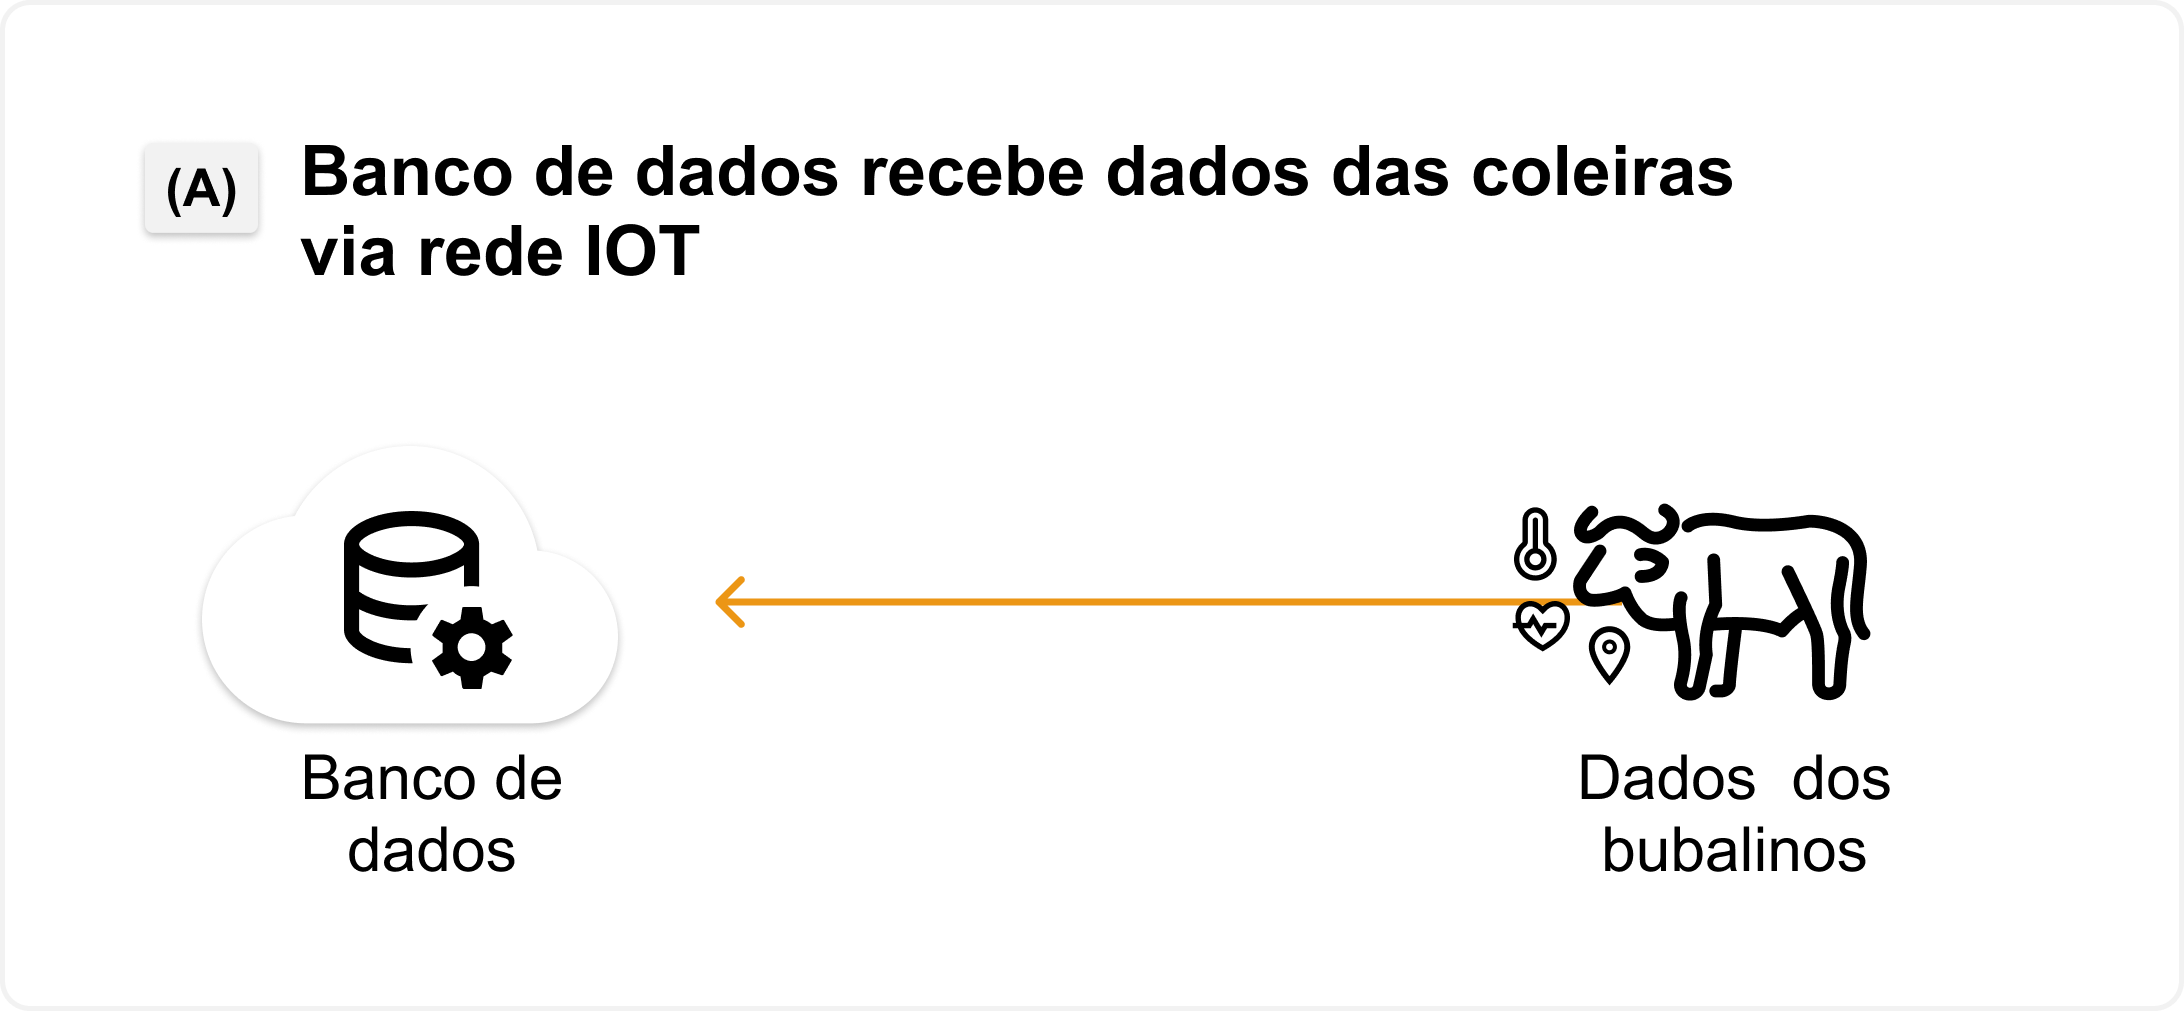
\includegraphics[width=\textwidth]{imgs/bubatag/A.png}
    \end{minipage}
    \hfill
    \begin{minipage}[c]{0.48\textwidth}
        \centering
        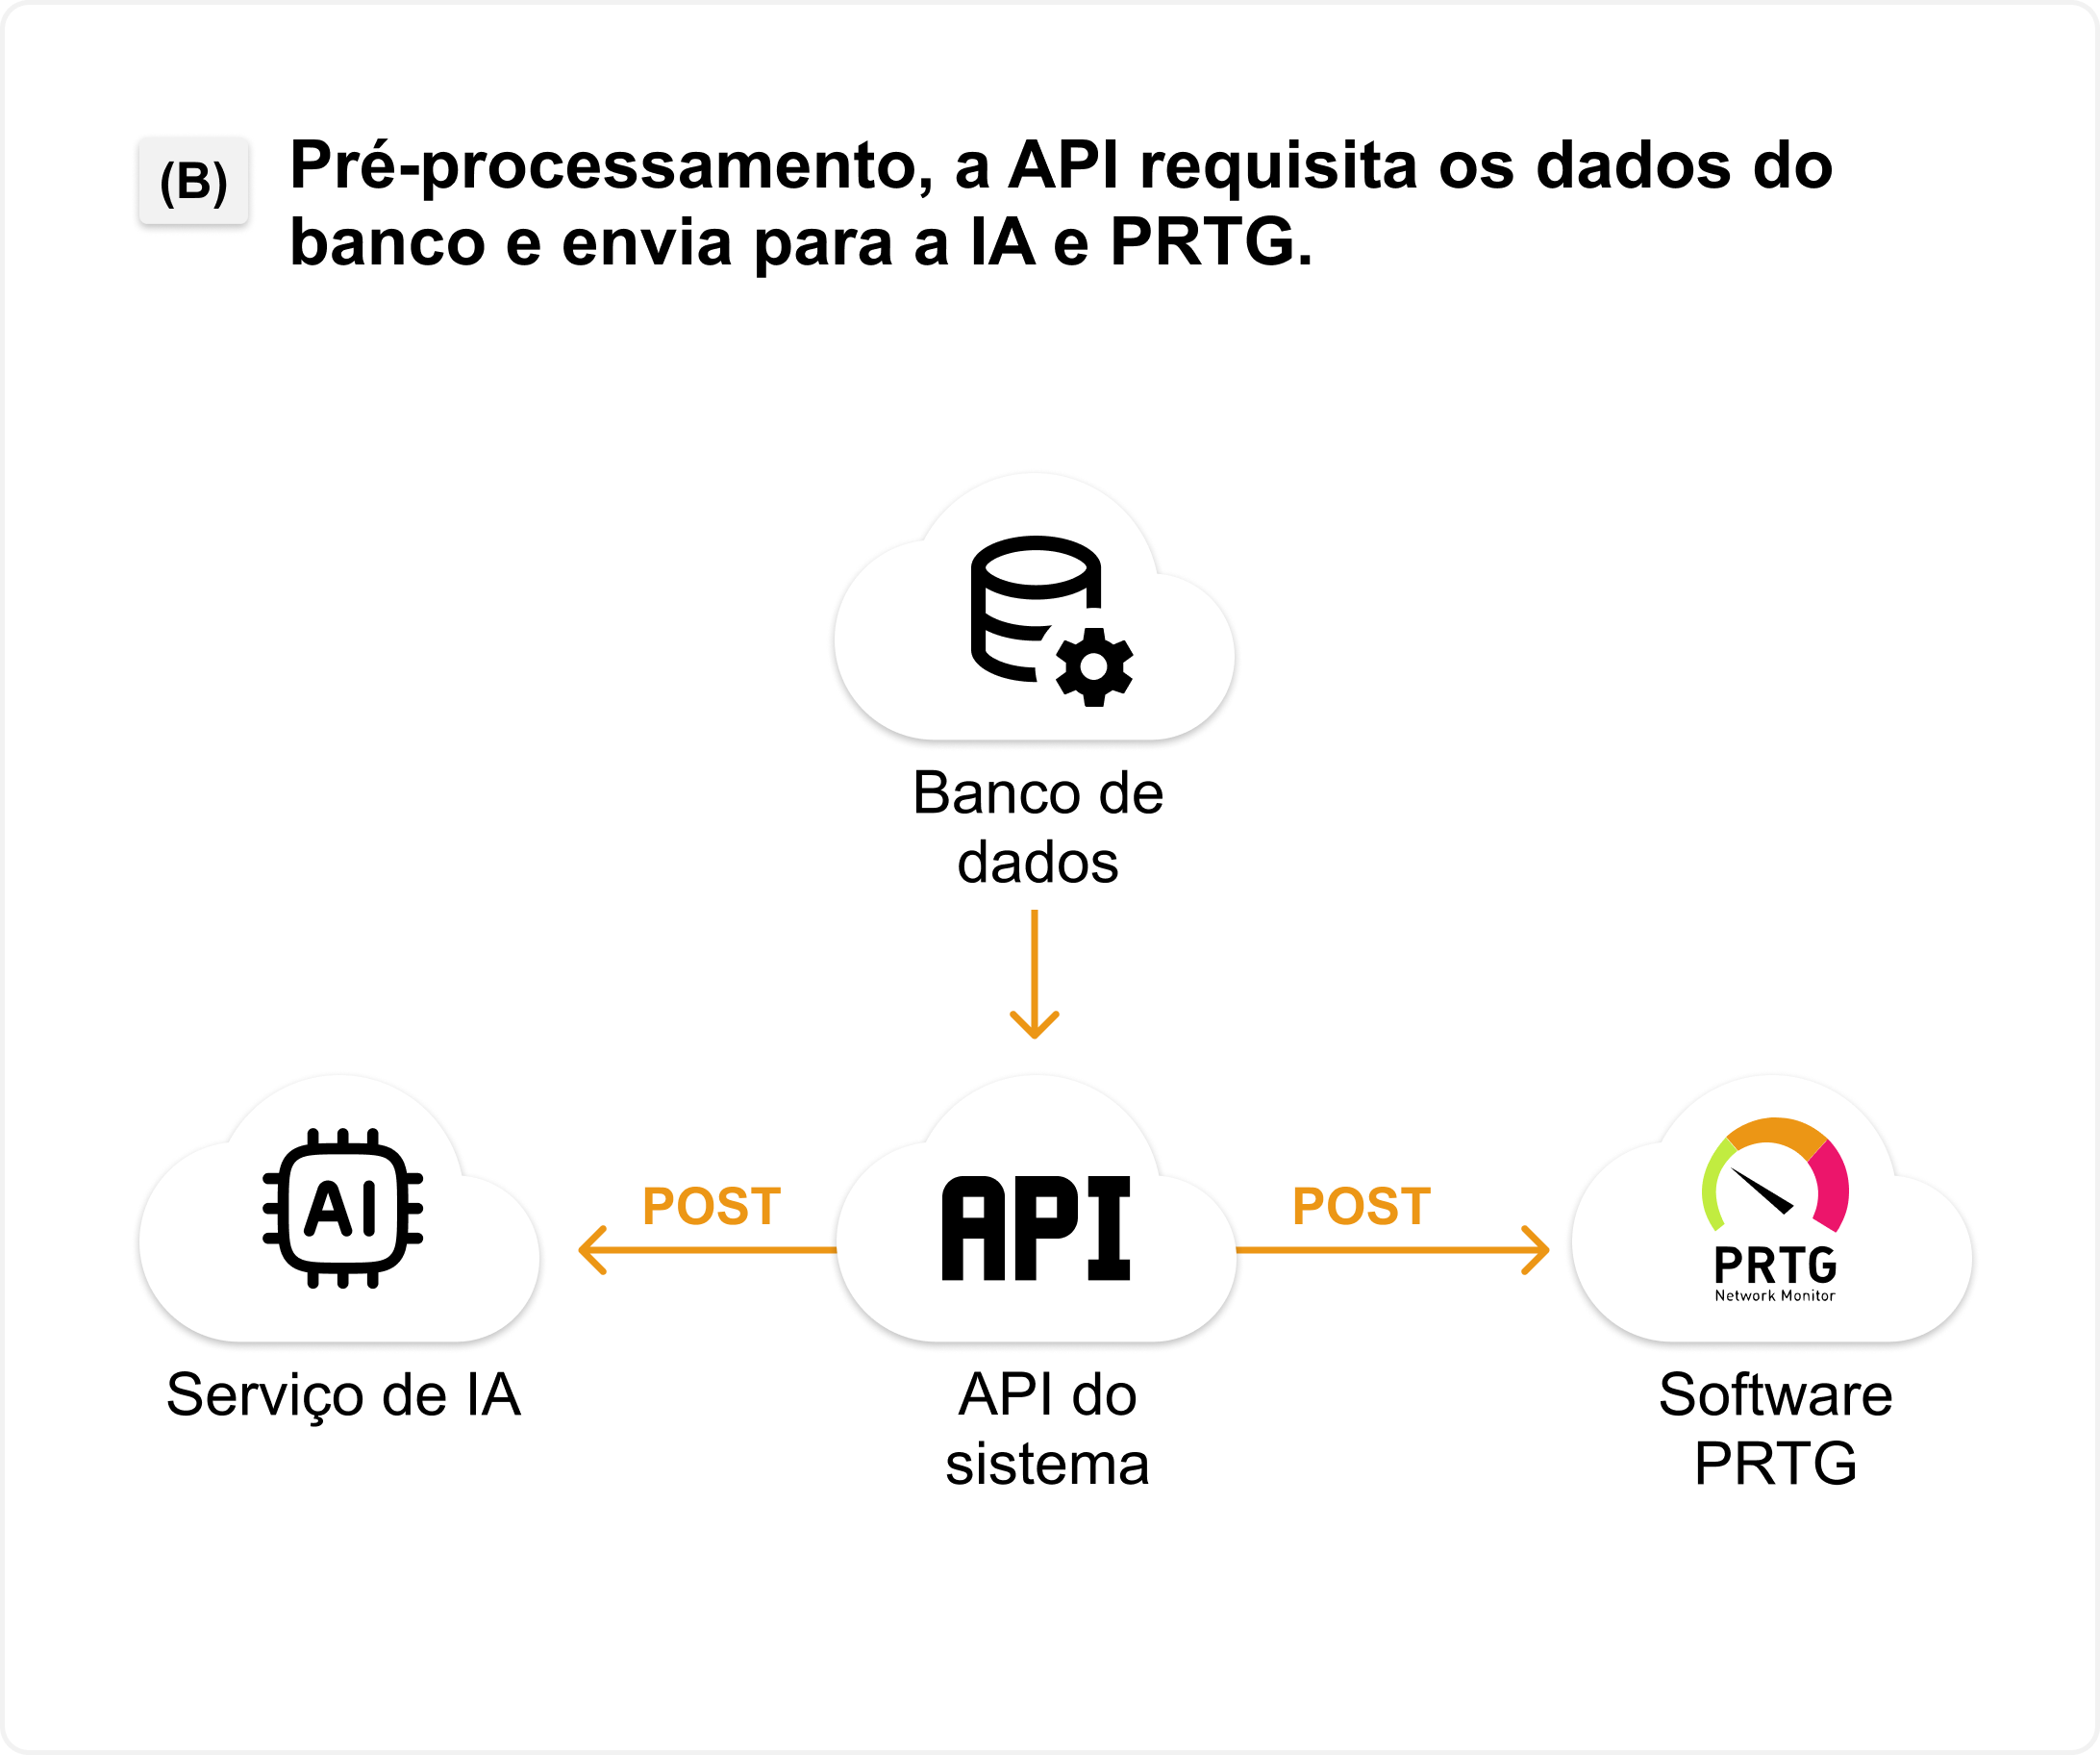
\includegraphics[width=\textwidth]{imgs/bubatag/B.png}
    \end{minipage}

    \vspace{0.2cm} % Espaço reduzido entre as linhas

    % Segunda linha (C e D)
    \begin{minipage}[c]{0.48\textwidth}
        \centering
        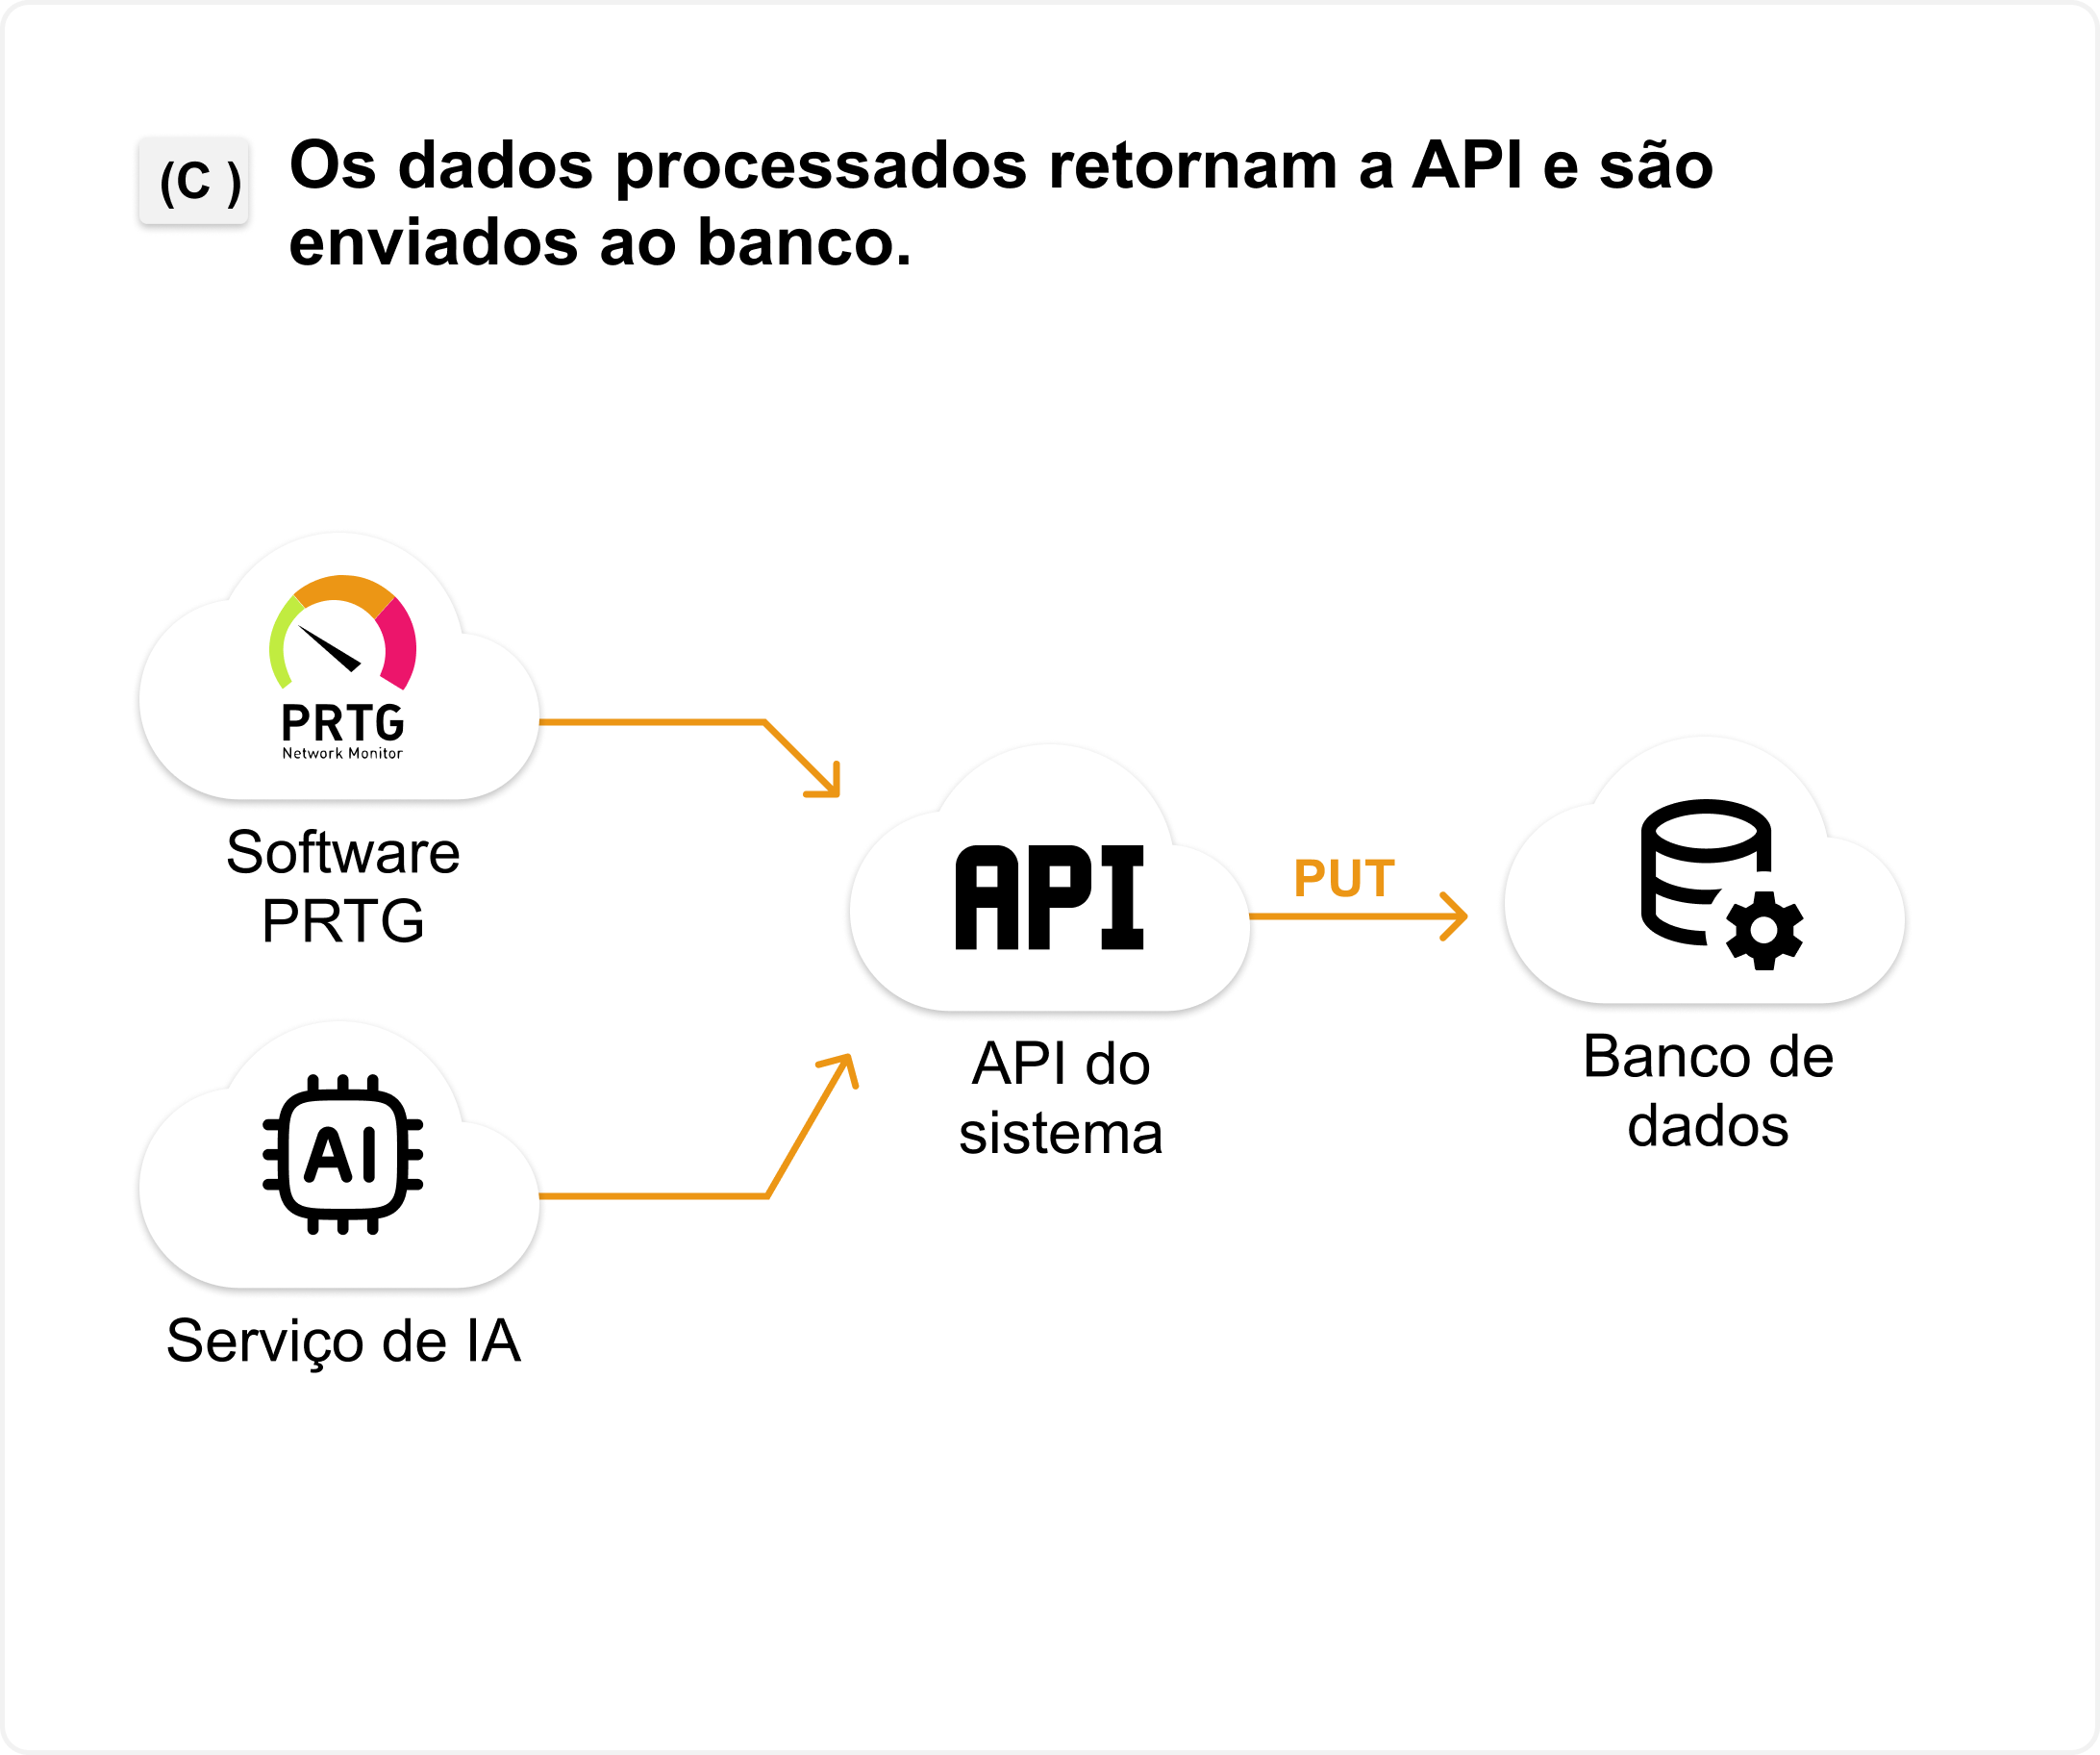
\includegraphics[width=\textwidth]{imgs/bubatag/C.png}
    \end{minipage}
    \hfill
    \begin{minipage}[c]{0.48\textwidth}
        \centering
        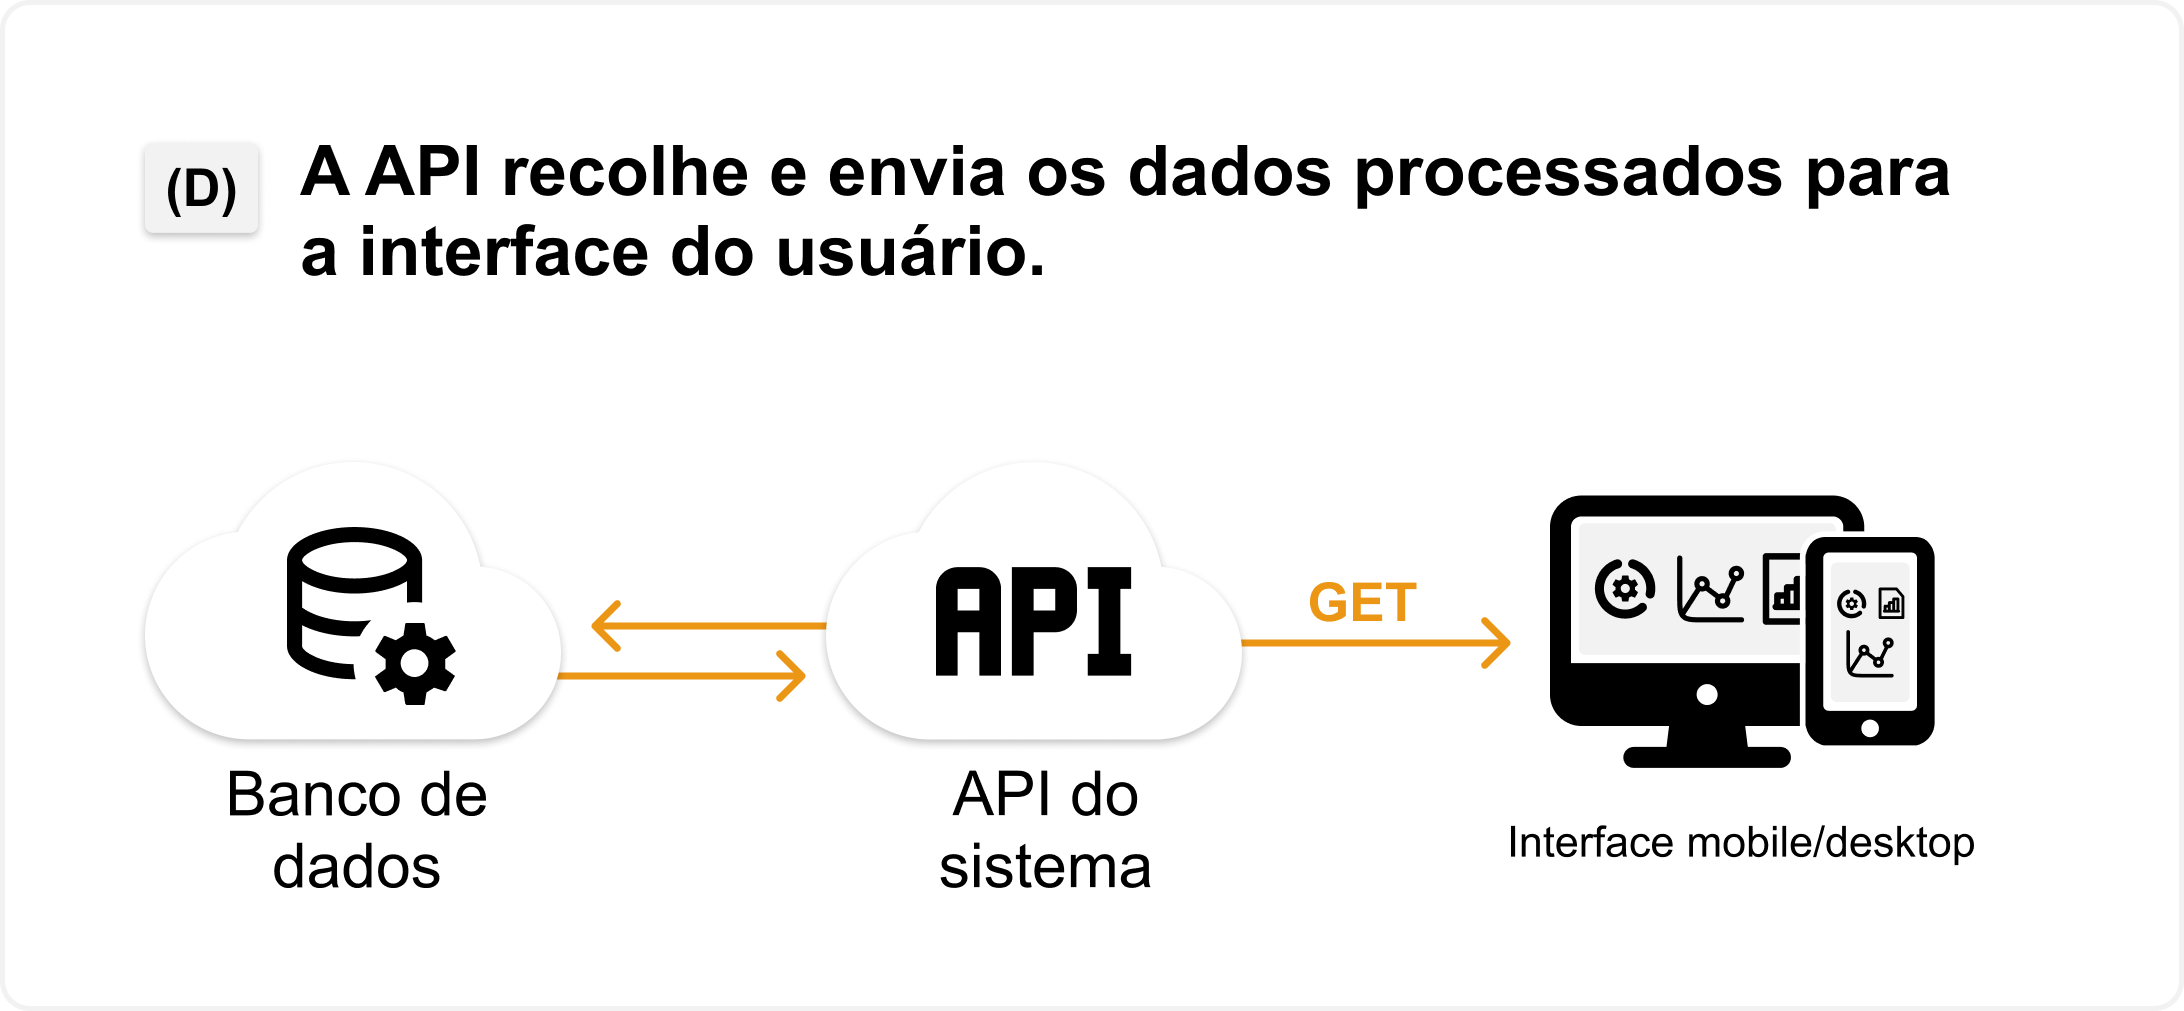
\includegraphics[width=\textwidth]{imgs/bubatag/D.png}
    \end{minipage}
    
    \caption{Fluxo de funcionamento da API.}
    \label{fig:fluxo_api}
\end{figure}

Os serviços externos, como a Inteligência Artificial (IA) e o PRTG, consomem os dados expostos pela API para realizar o processamento e o monitoramento. A IA atua classificando os
níveis de estresse de cada animal individualmente, enquanto o PRTG monitora o estado dos
dispositivos e a conectividade das coleiras, representando a Etapa B. Após o processamento realizado por esses serviços, na Etapa C,a API recebe os resultados (os níveis de estresse e o estado
operacional dos componentes) e atualiza o banco de dados com as informações processadas. Por
fim, na Etapa D, a API disponibiliza os dados consolidados e atualizados aos aplicativos móvel
e desktop, permitindo o acesso e a visualização pelo usuário final.



\subsection*{APLICATIVO MOBILE}

O aplicativo móvel foi projetado para ser simples, leve e de alta performance, permitindo que os
usuários acessem informações essenciais em qualquer área da fazenda. O foco principal está em
fornecer dados concisos e de fácil visualização, incluindo:

• Localização em tempo real dos animais: apresenta uma marcação no mapa da fazenda
indicando o ponto exato onde cada animal se encontra. Além disso, é exibida uma lista
com todos os animais cadastrados no sistema, acompanhada dos seguintes dados: ID do
animal (controle interno do sistema), etiqueta do animal (identificação da fazenda), número
do dispositivo (coleira eletrônica) e status do animal, representado por cores para facilitar
a interpretação visual — verde indica que o animal não está estressado e encontra-se dentro
dos limites impostos na fazenda, enquanto vermelho indica níveis elevados de estresse. Um
exemplo do protótipo desenvolvido no Figma pode ser visualizado na Figura 3.

• Monitoramento de temperatura e batimentos cardíacos: exibe, em tempo real, os níveis
de temperatura corporal (°C) e batimentos cardíacos (BPM) dos animais. Um protótipo
dessa funcionalidade pode ser observado na Figura 4. Essa tela funciona como uma ficha
individual do animal, diferenciada pela etiqueta de identificação (neste exemplo, o animal
TE18). Nela constam informações detalhadas, como batimentos cardíacos, temperatura,
nome, sexo, idade e histórico, permitindo ao usuário identificar rapidamente qual animal
está sendo monitorado.

\addtocounter{figure}{0} % Força o número da figura a avançar para o próximo (3)
\begin{figure}[H]
    \centering
    \caption{Tela de aplicativo mobile com localização de todos os animais cadastrados no sistema.}
    \label{fig:tela_mobile_localizacao}
    \vspace{0.3cm} % Espaço opcional entre a legenda e a imagem
    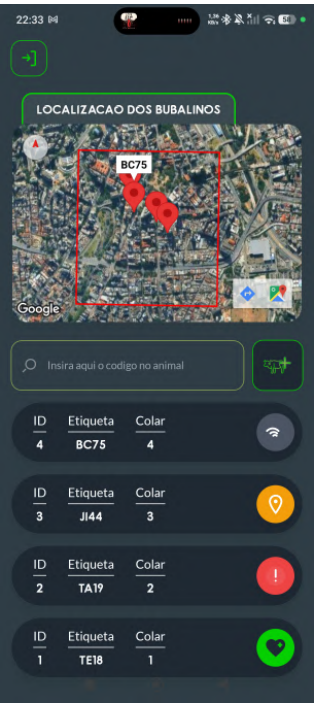
\includegraphics[width=0.45\textwidth]{imgs/bubatag/tela_mobile.png}
\end{figure}

\addtocounter{figure}{0} % Força o número da figura a avançar para o próximo (3)
\begin{figure}[H]
    \centering
    \caption{Tela protótipo de aplicativo mobile com as informações de estresse e dados do animal
específico (Etiqueta - TE18) cadastradas no sistema.}
    \label{fig:tela_mobile_localizacao}
    \vspace{0.3cm} % Espaço opcional entre a legenda e a imagem
    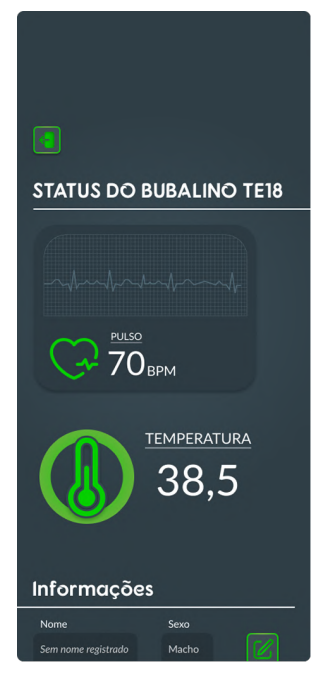
\includegraphics[width=0.45\textwidth]{imgs/bubatag/status.png}
\end{figure}

A simplicidade e o desempenho são fundamentais para garantir a usabilidade em áreas remotas ou com conectividade limitada.

\subsection*{PLATAFORMA WEB/DESKTOP}

O aplicativo desktop foi desenvolvido em JavaScript, utilizando o framework Node.js no backend. No front-end, foram empregados React e Tailwind CSS (Tailwind Cascading Style Sheets),
com o objetivo de criar uma ferramenta completa para o gerenciamento da fazenda, oferecendo
recursos avançados de visualização e análise de dados. As principais funcionalidades incluem:

• Visualização em tempo real de dados

• Histórico de estresse dos animais

• Histórico de localização dos animais

• Anotações personalizadas para cada animal (Figura 5)

Essas funcionalidades permitem que os usuários monitorem e gerenciem seus rebanhos de
forma mais eficaz, tomando decisões informadas com base em dados precisos e atualizados. Na
Figura 6, é possível visualizar o número total de animais e de coleiras cadastradas no sistema.
Além disso, a tela apresenta um resumo dos dados de estresse dos animais, incluindo o número
de animais estressados e não estressados, bem como a porcentagem de cada categoria em relação
ao total do rebanho. Essa visão geral permite ao usuário identificar rapidamente a situação do
rebanho e tomar decisões informadas para melhorar o manejo e o bem-estar dos animais.

\addtocounter{figure}{0} % Força o número da figura a avançar para o próximo (3)
\begin{figure}[H]
    \centering
    \caption{ Tela do aplicativo desktop, com as informações dos animais cadastrados no sistema.}
    \label{fig:tela_mobile_localizacao}
    \vspace{0.3cm} % Espaço opcional entre a legenda e a imagem
    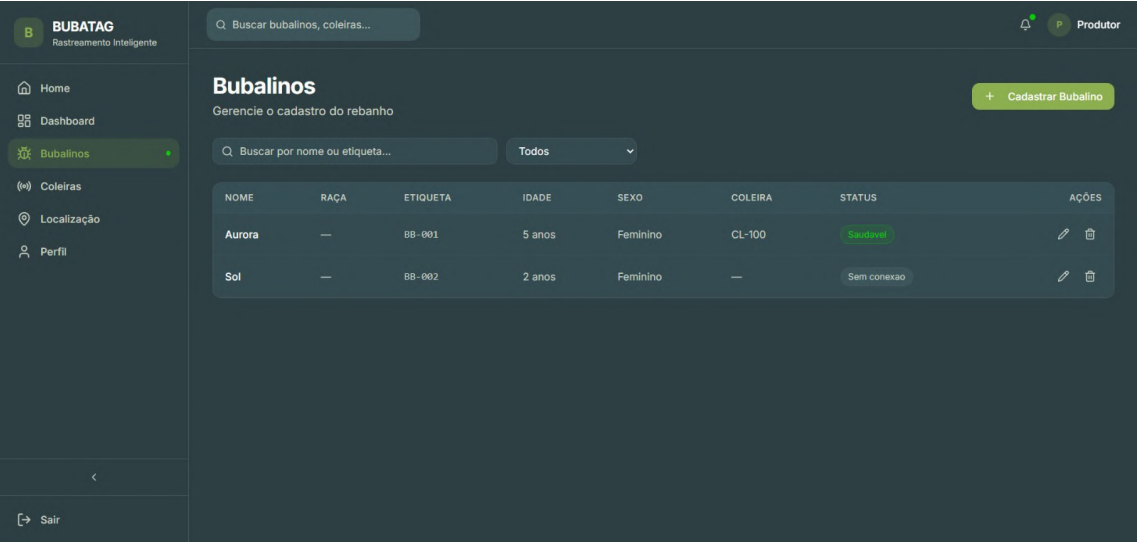
\includegraphics[width=0.90\textwidth]{imgs/bubatag/crud-bubalinos.png}
\end{figure}

\addtocounter{figure}{0} % Força o número da figura a avançar para o próximo (3)
\begin{figure}[H]
    \centering
    \caption{ Tela inicial do sistema desktop, com os dados principais resumidos.}
    \label{fig:tela_mobile_localizacao}
    \vspace{0.3cm} % Espaço opcional entre a legenda e a imagem
    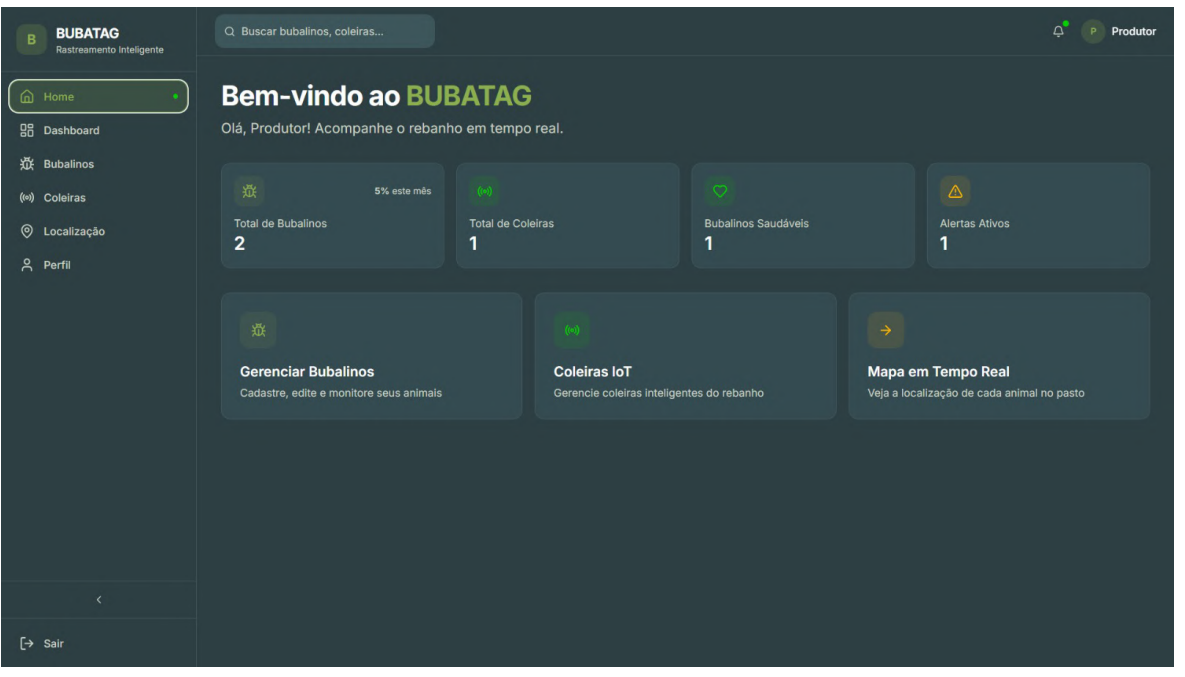
\includegraphics[width=0.85\textwidth]{imgs/bubatag/crud-home.png}
\end{figure}

Com o desenvolvimento dessas funcionalidades, a plataforma web/desktop oferece uma solução robusta e intuitiva para o monitoramento e gestão de rebanhos, contribuindo para a melhoria
do bem-estar animal e a eficiência produtiva na bubalinocultura.


% Referências
\nocite{*} % <--- Adicione esta linha para forçar a exibição de todas as referências
\bibliographystyle{IEEEtran}
\bibliography{referencias}

\end{document}

